Divergence from the counterintuitive behavior of regularization in TD also occurs in neural networks, as do vacuous models. We illustrate these over 100 separate initializations:
\begin{center}
    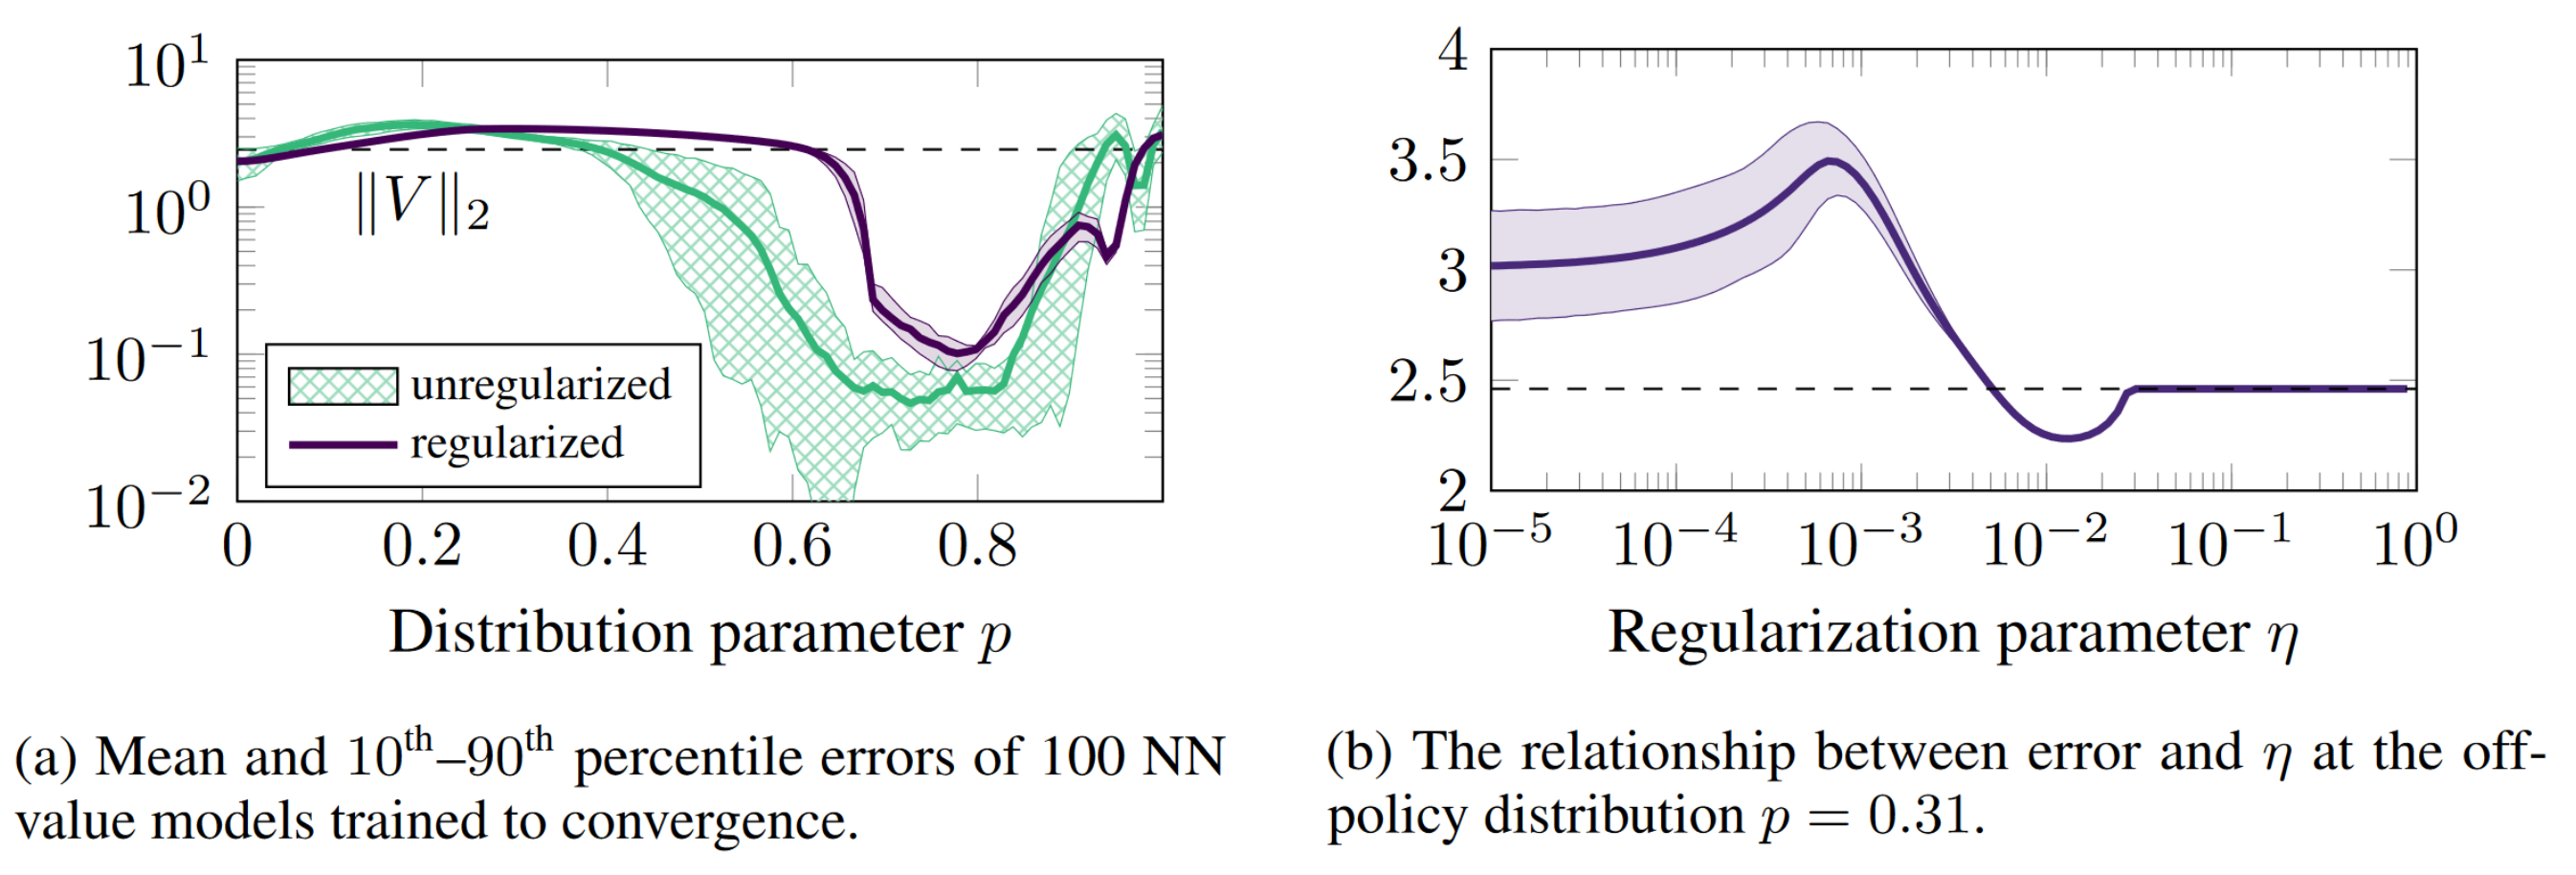
\includegraphics[scale=0.4]{parts/nn/nn2.png}
\end{center}
In (a), we show that, for some off-policy distributions, NNs can be vacuous. In (b), we show plot the relationship between TD error and regularization. All trained models exhibit a bump in error at similar levels of regularization, showing that this divergence is not an artifact of poor initialization.
